
\chapter{Neural Networks}
\label{ch:NN}









\index{Perceptron architecture}
\epigraph{On being asked, ``How is Perceptron performing today?'' I am often tempted to respond, ``Very well, thank you, and how are Neutron and Electron behaving?''}{Frank Rosenblatt, inventor of the perceptron and also the Perceptron  \cite{rosenblatt1961principles}.\index{Rosenblatt, Frank}}



\noindent{}With our mathematical lessons concluded, we turn to an introductory overview of deep learning.

In~\S\ref{sec:MLP_intro}, we introduce the basic components of neural network architectures -- neurons, activations, biases, weights, and layers -- in order to define the \emph{multilayer perceptron} (MLP),
a simple model that is iteratively composed of these basic components.  Given that all deep networks are by definition iteratively composed of many structurally identical layers, MLPs will play the role of archetype network architecture for illustrating the principles of deep learning throughout the book.
This class of neural-network models is rich enough to capture all the essential aspects of deep learning theory, while simple enough to maintain the pedagogical focus of the book. Nevertheless,
we'll also briefly comment on how one could work out an effective theory for other network architectures.

In~\S\ref{sec:activations} we list some common activation functions that are 
often used in practice.

Finally, we discuss in~\S\ref{sec:MLP_distribution} how MLPs are initialized. %
Here, we make a key conceptual shift from thinking about the weights and biases as the random variables
to thinking about the induced distribution over the neural activities and network outputs.
The expressions we derive here will provide a natural starting point for our analysis in~\S\ref{ch:ngp} when we start developing our effective theory of MLPs with general activation functions.




\section{Function Approximation}\label{sec:MLP_intro}


\index{neural network}
The subject of \emph{artificial neural networks}\index{artificial neural network|see{neural network}} has a rich history as \terminate{cognitive science} and \terminate{neuroscience}--inspired
\terminate{artificial intelligence}.\footnote{The \neo{artificial neuron} was invented by McCulloch and Pitts in 1943 \cite{mcculloch1943logical} as a model of the \neo{biological neuron}. Their neuron was essentially a perceptron with a bias, but did not have learnable weights. The perceptron model\index{Perceptron architecture}, with learnable weights, was invented by Rosenblatt in 1958 \cite{rosenblatt1958perceptron}.
Deep learning 
really came into its own
in 2012~\cite{ImageNet2012} after the realization that the \terminate{graphical processing unit}\index{GPU|see{graphical processing unit}} (GPU) is well-suited for the parallel computations required to train and run neural networks.\index{deep learning!history}\index{neural network!history}} Here, our starting point will be a discussion of the function, $f(x)$.

\index{Taylor series}
Some functions are really simple, %
easily described in terms of the elementary operations\index{elementary operation}: addition, subtraction, multiplication, and division.
For instance, consider either the identity function $f(x)=x$ or the exponential function $f(x)=e^{x}$. The former is the definition of trivial, involving no operations. The latter is a special function and can be defined in many ways, e.g.~through its Taylor series
\be\label{eq:exponential-Taylor-expansion}
e^{x}\equiv\sum_{k=0}^\infty \frac{x^k}{k!}\, .
\ee
This definition constructs the exponential function in terms of elementary operations of addition, multiplication, and division: the numerator $x^k$ represents the repeated multiplication of the variable $x$ for $k$ times, and the factorial $k!$ in the denominator represents the repeated multiplication of integers $k!=1 \times 2 \times \cdots \times (k-1) \times k$. Although this description of the exponential function involves a sum of an infinite number of terms, the actual instructions~\eqref{eq:exponential-Taylor-expansion} for computing this function in terms of these simple operations are so compact that they takes up only about one seventh of a line and, for many purposes, it only takes the first few terms in the sum
to get a
useful approximation of $e^x$.

Some functions are really complicated and their description in terms of elementary operations is unlikely to fit in the confines of any printed book. For instance, imagine a function $f(x)$ that takes as input an image $x_i$ 
-- represented as a vector of numbers corresponding to a black-and-white pixelated image -- 
and outputs $1$ if the image $x_i$ depicts a cat and $0$ otherwise. While such a classification function should exist since humans can recognize images of cats, it's not at all clear how to describe such a function in terms of simple operations like addition and multiplication. The subject of \term{artificial intelligence} (AI) is mostly concerned with functions of this sort: easy for humans to compute, but difficult for humans to describe in terms of elementary operations. 


The conceptual leap needed to represent such hard-to-describe functions is to start with a flexible \emph{set} of functions $\le\{f(x;\theta)\ri\}$, constructed from simple components parametrized by a vector of adjustable \term{model parameters} $\theta_{\mu}$. One then tries to tune these model parameters $\theta_{\mu}$ judiciously in order to approximate the original complicated function such that $f(x;\theta^\star) \approx f(x)$. The description of the set of functions $\le\{ f(x;\theta)\ri\}$ as well as the settings of the model parameters $\theta^\star_{\mu}$ then serve as a useful approximate description of a desired function $f(x)$. This is called \term{function approximation} and the procedure for adjusting the model parameters $\theta_{\mu}$ is called a \term{learning algorithm}.%

\index{dataset|see{input data}}\index{input data|seealso{training set}}\index{input data|seealso{test set}}\index{input data|seealso{validation set}}
To be more concrete, let us represent the collection of 
inputs to our function $f(x)$ as a set $\D$ of $n_0$-dimensional vectors
\be
\D=\le\{\x{i}{\alpha}\ri\}_{\alpha=1,\ldots,\ND}\, ,
\ee
called \textbf{input data}.
Here, the \textbf{sample index} $\alpha$ labels each sample in the dataset of $\ND$ elements, and the vector index $i=1,\ldots,n_0$ labels the component of the input vector. 
In our motivating example above, each number $\x{i}{\alpha}$ refers to the $i$-th pixel
of the $\alpha$-th  image in the dataset\index{input data|textbf} $\D$ of $\ND$ images, each of which might or might not 
depict a cat. By adjusting the model parameters $\theta_{\mu}$ so that the function $f(x;\theta^\star)$ outputs the correct answer for as much input data as possible, we can try to approximate the elusive cat-or-not %
function in a way that no longer defies description. The overall idea of \neo{training} such functions using a dataset $\D$ -- rather than \neo{programming} them --  goes by the name \term{machine learning}\index{machine learning|seealso{statistics (branch of mathematics)}}
and stands in contrast to the conventional von Neumann\index{von Neumann, John} model of the digital computer. \index{sample indices}


\index{function approximation}\index{artificial intelligence}\index{deep learning}
While any set of parameterized functions can be used for function approximation,\footnote{\index{Gaussian function}E.g.~consider a sum of  Gaussian functions, where the mean and variance of each Gaussian play the role of the adjustable parameters.} our focus will be on a particular set of composable functions originally derived from a simplified model of the \terminate{brain}. Such functions were originally termed \textbf{artificial neural networks} and are now just referred to as \textbf{neural networks}\index{neural network|textbf}. \textbf{Deep learning} is a branch of machine learning that uses neural networks as function approximators, with a particular emphasis on stacking \emph{many layers} of structurally similar components. Let's see how this works in more detail.






\index{biological neuron}\index{artificial neuron}
The most basic component of the neural network is the \term{neuron}. Loosely inspired by the behavior of biological neurons, the artificial neuron essentially consists of two simple operations:
\bi
\item The \term{preactivation} $z_i$ of a neuron is a linear aggregation of 
incoming signals $s_j$ where each signal is weighted by $W_{ij}$ and
biased by $b_i$
\be\label{eq:preactivation}
z_{i}(s) = b_i+\sum_{j=1}^{n_{\text{in}}}W_{ij}\, s_{j}\,  \quad \text{for} \quad i=1,\ldots,n_{\text{out}}\, .
\ee
\item Each neuron then \emph{fires} or not according to the weighted and biased evidence, i.e.~according to the value of the preactivation $z_i$, and produces an \term{activation}
\be
\sigma_i \equiv \sigma\!\le(z_{i}\ri) \, .
\ee
The scalar-valued function $\sigma(z)$ is called the \term{activation function} and acts independently on each component of the preactivation vector.
\ei
Taken together, these  $n_{\text{out}}$ neurons form a \term{layer}, which takes in the $n_{\text{in}}$-dimensional vector of signals $s_j$ and outputs the $n_{\text{out}}$-dimensional vector of  activations $\sigma_i$.   With this collective perspective, a layer is parameterized by a vector of \term{biases} $b_i$ and a matrix of \term{weights} $W_{ij}$, where $i=1,\ldots,n_{\text{out}}$ and $j=1,\ldots,n_{\text{in}}$, together with a fixed activation function $\sigma(z)$.\index{weights|seealso{model parameters}}\index{biases|seealso{model parameters}}

With these components, we can make an increasingly flexible set of functions by organizing many neurons into a layer and then iteratively stacking many such layers, so that the outgoing activations of the neurons in one layer become the input signals to the neurons in some other layer.
The organization of the neurons and their pattern of connections is known as the neural network \term{architecture}.
The archetypical neural network architecture based on this principle of stacking 
layers of many neurons is called the \term{multilayer perceptron} (MLP).\footnote{Here, the name ``perceptron''\index{perceptron|see{Perceptron architecture}} was inherited from Rosenblatt's Perceptron architecture\index{Perceptron architecture} \cite{rosenblatt1958perceptron}, which was originally envisioned for emulating \neo{human perception}. The name perceptron is also used to refer to the original step-function activation function, cf.~the first entry of \S\ref{sec:activations}. 
    \index{activation function!perceptron@$\texttt{perceptron}$}
} 

The activation function is usually chosen to be a nonlinear function in order to increase the \terminate{expressivity}
of the neural-network function $f(x;\theta)$.
The simplest -- and historically first -- activation function either fires or does not fire: $\sigma(z) =1$ for $z\geq0$ and $\sigma(z) =0$ for $z<0$. In other words, each neuron fires if and only if the weighted accumulated evidence $\sum_jW_{ij}\, x_{j}$ exceeds the firing threshold $-b_i$. More generally, activation functions are not binary and can incorporate
the strength of the evidence into their output. In~\S\ref{sec:activations} we'll describe many of the commonly-used activation functions in deep learning. 

\begin{figure}
\begin{center}
 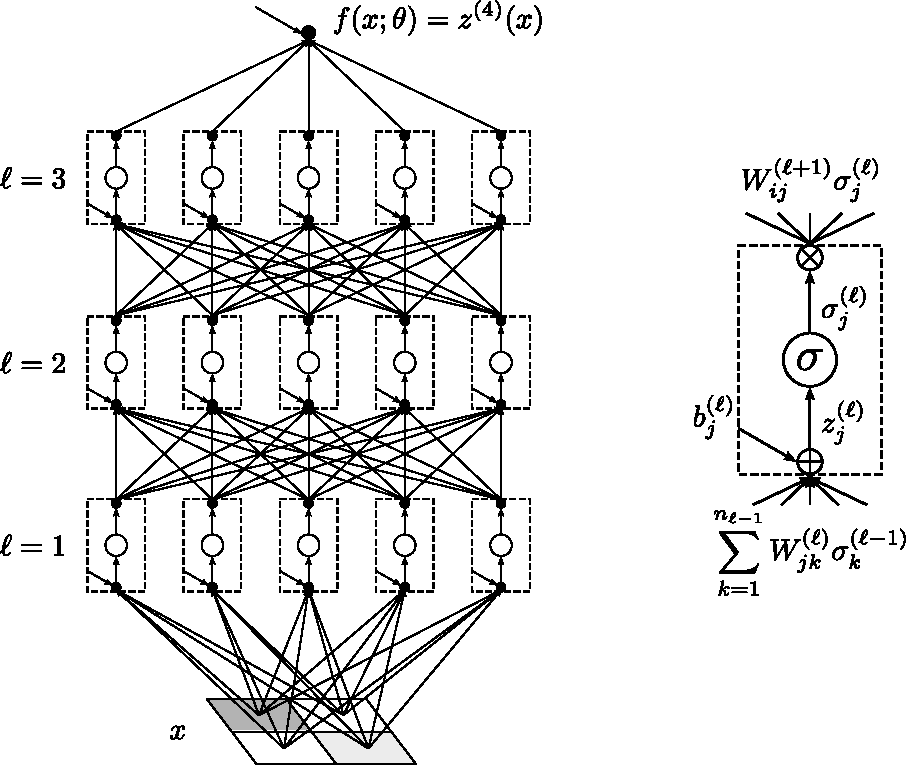
\includegraphics[width=.9\linewidth]{./book_figures/mlp.pdf}
\caption{
\textbf{Left:} depiction of the neurons and connections for an example \terminate{multilayer perceptron} (MLP) architecture.  This particular MLP has $L=4$ layers, defining a set of functions $f(x; \theta)$ with input dimension $n_0=4$ and output dimension $n_{4}=1$. The three hidden layers have five neurons each $n_1, n_2, n_3 = 5$, implying $P=91$ total model parameters. 
The graph describing the connections between neurons is a \neo{directed acyclic graph}, meaning that signals only propagate in one direction and do not loop inside the network.
For this reason, MLPs are also sometimes called \emph{feedforward} networks\index{feedforward network}.
\textbf{Right:} the detailed structure of each \terminate{neuron} that \emph{(i)} adds the bias 
and the weighted signals 
to produce the preactivation, 
\emph{(ii)} generates the activation 
from the preactivation, and \emph{(iii)} multiplies the activation by the next-layer weight.
}
\label{fig:ff-example}
\end{center}
\end{figure}


\index{function approximation}\index{model parameters}\index{FCN|see{fully-connected network}}\index{fully-connected network|seealso{multilayer perceptron}}
The MLP is recursively defined through the following iteration equations
\begin{align}\label{eq:mlp-definition}
&z_i^{(1)}(x_\alpha)\equiv\bias{i}{1}+\sum_{j=1}^{n_{0}}\W{ij}{1}\x{j}{\alpha}\,, \quad \text{for} \quad i=1,\ldots,n_1\, ,\, \\
&z_i^{(\ell+1)}(x_\alpha)\equiv\bias{i}{\ell+1}+\sum_{j=1}^{n_{\ell}}\W{ij}{\ell+1}\sigma\!\le(z_j^{(\ell)}(x_\alpha)\ri)\, , \quad \text{for} \quad i=1,\ldots,n_{\ell+1}\, ;~ \ell=1,\ldots,L-1\, , \notag
\end{align}
which describes a network with $L$ layers of neurons, with each layer $\ell$ composed of $n_\ell$ neurons.\footnote{
 A more modern name for the MLP is the \neo{fully-connected network} (FCN),
highlighting the fact that each neuron in a given layer $\ell$ has a connection to every neuron in layer $\ell+1$, as Figure~\ref{fig:ff-example} makes clear. Such a dense pattern of connections is computationally expensive in terms of the number of parameters required for the architecture and should be contrasted with the sparser architectures described at the end of this section.
To place an emphasis on the \emph{deepness} of networks rather than on the \emph{density} of the connections, we'll mainly stick with the name \emph{multilayer} perceptron over the name \emph{fully-connected} network in this book.\index{multilayer perceptron!a.k.a.~a fully-connected network}
}
We depict an example MLP architecture in Figure~\ref{fig:ff-example}. The number of layers $L$ defines the \term{depth} of the network and the different number of neurons in each layer $n_{\ell=1,\ldots,L-1}$ define the \textbf{widths}\index{width|textbf} of the layers.
The depth and hidden-layer widths are variable \term{architecture hyperparameters} that define the shape of the network, while the values of $n_0$ and $n_{L}$ are set by input and output dimensions of the function-approximation task, respectively.
In particular, the final-layer preactivations computed by the network
\be
f\!\le(x; \theta\ri) = z^{(L)}(x),
\ee
serves as the function approximator, with its model parameters $\theta_{\mu}$ being the union of the biases and weights from all the layers. Sometimes it will be convenient to think of this collection of model parameters as an explicit vector $\theta_\mu$ whose components cover all the model parameters.
In that case, the dimension of $\theta_\mu$ and therefore the total number of the model parameters is given
by
\be
P = \sum_{\ell=1}^{L} \le(n_{\ell} + n_{\ell}n_{\ell-1} \ri) \, ,
\ee
which scales quadratically with the widths of the network and linearly with the depth.


The intermediate layers $\ell= 1, \dots, L-1$ are referred to as \textbf{hidden layers}\index{hidden layer|textbf}, since preactivations and activations of the neurons from those layers are not part of the network's output. On the one hand, the variables $z^{(\ell)}(x)$ for $\ell < L$ are simply temporary variables introduced to construct
an increasingly flexible set of functions, expressive enough to have a chance of approximating hard-to-describe functions.
On the other hand, in analogy to the physical \terminate{brain}, these variables are thought to encode 
useful information about \emph{how} the \terminate{neural network} is approximating; for example, a particular neuron might fire if it recognizes a tail, a whisker, or a pattern representing fur -- all potentially useful \emph{features}\index{feature}\index{feature|seealso{representation}}
for determining whether an image contains a cat or not.










\index{architecture}\index{inductive bias!of model architectures}\index{convolutional neural network|textbf}
Moving beyond MLPs, the choice of neural network architecture is often motivated by the nature of the function we are trying to approximate. For instance, the properties of the dataset\index{input data} $\D$, when known and articulated, can be used to build \textbf{inductive biases} into the architecture so that the resulting set of functions may better represent the underlying function.\footnote{We'll discuss the inductive bias of MLPs from various different perspectives in 
\S\ref{ch:bayesian-inference}, \S\ref{ch:features}, and Epilogue~\ref{epi:overparameterization}.} 
Let's look at a few examples.
\bi
\item For \term{computer vision} (CV) applications, \textbf{convolutional neural networks} (CNN) or conv-nets~\cite{fukushima1980neocognitron,lecun89conv,LeCunZipCode1989,lecun1998gradient,ImageNet2012} are used to take advantage of the fact that information in images is organized in a spatially local manner, often respecting \neo{translational invariance}.\footnote{
For a two-dimensional convolutional layer, the iteration equation~\eqref{eq:mlp-definition} for MLPs is replaced by
\be
\label{eq:conv-layer}
z_{i,(c,d)}^{(\ell+1)}(x_\alpha)\equiv\bias{i}{\ell+1}+\sum_{j=1}^{n_{\ell}}\sum_{c'=-k}^{k}\sum_{d'=-k}^{k}\W{ij}{\ell+1}\sigma\!\le(z_{j,(c+c',d+d')}^{(\ell)}(x_\alpha)\ri)\, ,
\ee
where in $z_{i,(c,d)}^{(\ell)}$, the first index $i$ is an auxiliary \neo{channel}\index{channel|seealso{convolutional neural network}} index and the paired index $(c,d)$ is a two-dimensional spatial index, and the number $k$ is a fixed constant for each layer, determining the size of the convolutional window. In particular, the same weights are used on different spatial locations of the input, which promotes the inductive bias that image data are often translationally invariant. In other words,
a cat is still a cat regardless of its location in an image.
At the time of writing, the convolutional layer is an essential part of many modern deep learning architectures, but this situation may change in the future. Please pay \neo{attention}.
}
\item For \term{natural language processing} (NLP) applications, the \term{transformer} architecture (no acronym yet) is used to process sequential input -- such as a paragraph of text or an amino acid sequence coding a protein -- in a way that encourages correlations to develop between any of the elements in the sequence \cite{attention2017}. This property of the model is aptly called \neo{attention}.\index{language model}\index{attention|seealso{transformer}}
\ei
An important property of these inductive biases is that they induce constraints or relationships between the weights. For instance, we can think of the convolutional layer as a particular type of MLP layer, where many weights are set to zero and the values of remaining weights are further shared among several different neurons. This property is known as \neo{weight tying}\index{weight tying|seealso{convolutional neural network}}. That means that convolutional layers are actually within the class of functions describable by using MLP layers, but they are very unlikely to be found via training unless the constraints are explicitly enforced. As long as the inductive bias of spatial locality and translational invariance is well founded, the convolution layer
has obvious computational advantages by heavily curtailing the number of weights to be trained and stored.

Regardless of these specific inductive biases ingrained into modern neural network architectures used in deep learning, the common thread to all is the idea of constructing a flexible set of functions by organizing neural components into many iterated layers. MLPs are the simplest of these neural network architectures that hinges on this stacking idea, and thus provide a \emph{minimal model}\index{minimal model!of deep learning} for an \term{effective theory of deep learning}.
Specifically, we expect that (\textit{a}) the \neo{principles of deep learning theory} that we uncover to be general and valid across the large variety of architectures that are based on the idea of stacking many layers of neural components and (\textit{b}) the resulting effective theory formalism can be specialized to specific architectures of interest as needed, using this book as a guide for how to work out such a theory. In particular, one can study other architectures in our formalism simply by swapping out the MLP iteration equation~\eqref{eq:mlp-definition} -- e.g.~for the convolution layer iteration equation~\eqref{eq:conv-layer} --  in the appropriate place. We'll provide pointers on where to make such substitutions when we begin working out our effective theory in~\S\ref{ch:ngp}. 

Finally, in Appendix~\ref{app:residual} we'll study neural networks with \emph{residual connections}\index{residual connection}, known as \textbf{residual networks}\index{residual network|textbf}. These architectures are specially modified to enable the training of deeper and deeper networks. In the final section of that appendix, we'll also explain how our effective theory approach\index{effective theory} can be extended to \emph{general} residual networks, including the \emph{residual convolutional network}\index{convolutional neural network!with residual connections|see{ResNet}} or \term{ResNet} and the \neo{transformer} architecture.

\index{RNN|see{recurrent neural network}}\index{CNN|see{convolutional neural network}}\index{MLP|see{multilayer perceptron}}\index{ConvNet|see{convolutional neural network}}












\section{Activation Functions}\label{sec:activations}
\begin{figure}\label{fig:activations}
\begin{center}
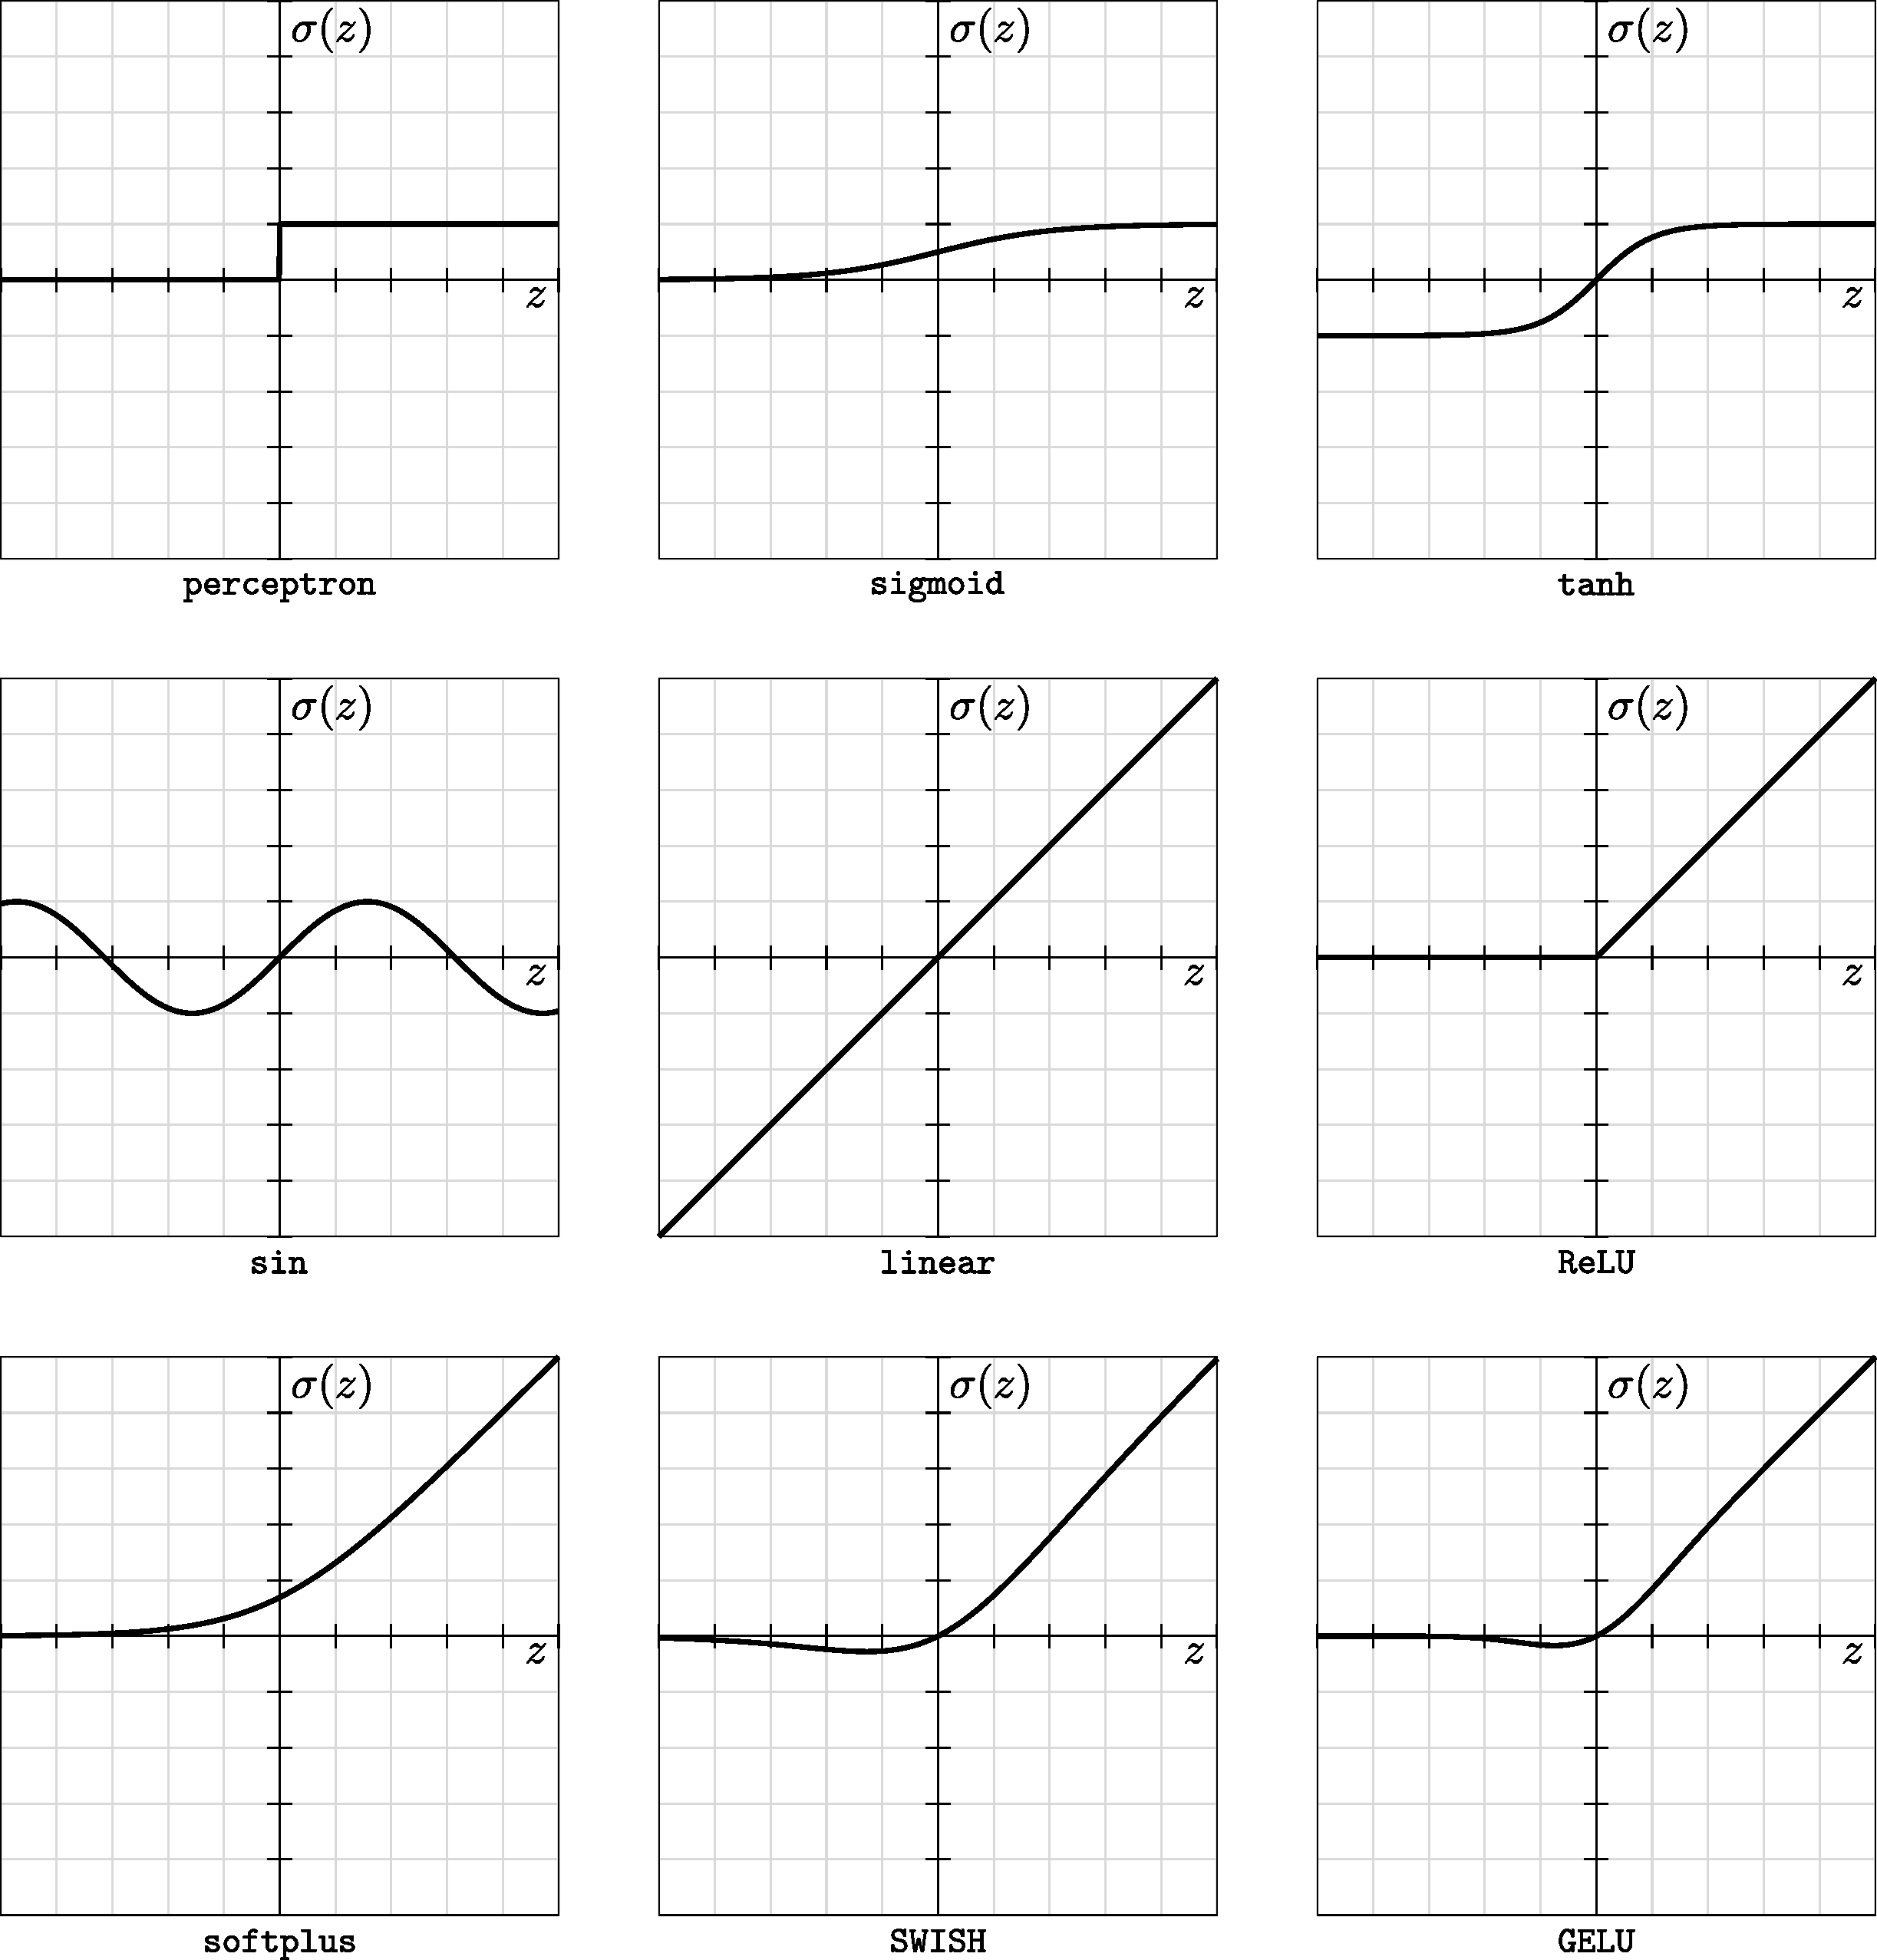
\includegraphics[width=.9\linewidth]{book_figures/activations/activations.pdf}
\caption{Commonly-used activation functions $\sigma(z)$. Grids are in units of one for both the preactivation $z$ and activation $\sigma$. 
(The $\lrelu$ is not shown.)}
\end{center}
\end{figure}
\index{activation function}
In this section, we discuss some of the most common activation functions. This list is non-exhaustive, so hopefully you won't find this section exhausting.
To make it easier for you, we've plotted all these activation functions together in Figure~\ref{fig:activations}. In \S\ref{ch:signalprop}, we'll use our effective theory to evaluate the relative usefulness of these activation functions in allowing input signals to effectively pass through a deep network.





\subsubsection{Perceptron}
The $\perc$ was the original activation function \cite{mcculloch1943logical}.\index{perceptron@$\texttt{perceptron}$|see{activation function}}
It is just a step function
\be
\sigma(z) = 
    \begin{cases}
    1\, , & z \ge 0  \, , \\
    0 \, , & z < 0 \, ,
    \end{cases}
\ee
corresponding to a computer scientist's notion of simplicity: the neuron either \emph{fires} and outputs $1$ or \emph{doesn't fire} and outputs $0$.\footnote{Alternatively, the $\perc$ may be shifted and scaled such that $\sigma(z)=\text{sign}(z)$.
}

Despite the logical simplicity, this turns out to be a poor choice. As we will see, in order to both effectively pass signals through networks (\S\ref{ch:signalprop} and \S\ref{ch:eft-ntk}) and train them~(\S\ref{ch:NTHb}), 
it's helpful to propagate more than one bit of information about the preactivation $z$. The $\perc$ has historical significance, but is never used in deep neural networks.


\subsubsection{Sigmoid}\index{sigmoid@$\texttt{sigmoid}$|see{activation function}}
The $\sigmoid$ activation function is a logistic function\index{logistic function}\index{logistic function|seealso{softmax distribution}}
\be\label{eq:sigmoid}
\sigma(z)=\frac{1}{1+e^{-z}} = \frac{1}{2}+\frac{1}{2}\tanh\!\le( \frac{z}{2}\ri)\, ,
\ee
which is a smoothed version of the $\perc$. Not only is it continuous, but also it preserves information about the magnitude of the preactivation, albeit mostly in the range near $z=0$ where the function is nearly linear. Outside of this range, the $\sigmoid$ heavily compresses such information as it becomes more and more $\perc$-like, \emph{saturating}\index{saturation (of an activation)} as $\sigma(z) = 1$ when $z \to \infty$ and as $\sigma(z) = 0$ when $z \to -\infty$.


As a mapping from the domain of $(-\infty,\infty)$ to the range $[0,1]$, the $\sigmoid$ also has a natural interpretation of converting log-odds to a probability, which is its main application in \terminate{machine learning}.
For \terminate{deep learning}, the differentiability of the $\sigmoid$ was essential in the development of a learning algorithm -- \terminate{backpropagation} -- for training neural networks with hidden layers \cite{rumelhart1985learning}. 
Nevertheless, the $\sigmoid$ activation function is still a poor choice %
in \emph{deep} neural networks:
as we'll see in~\S\ref{ch:signalprop}, a problem arises from the fact that it doesn't pass through the origin.







\subsubsection{Tanh}\index{tanh@$\texttt{tanh}$|see{activation function}}
The hyperbolic tangent or $\tanhA$ activation function
\be
\sigma(z) = \tanh(z) = \frac{e^z - e^{-z}}{e^z + e^{-z}} = \frac{e^{2z} - 1}{e^{2z} + 1} \, ,
\ee
is a scaled (both before and after the activation) and shifted $\sigmoid$, as is clear from~\eqref{eq:sigmoid}. Of particular importance is the fact that it's shifted such that $\sigma(0)=0$ \cite{lecun2012efficient}.


The $\tanhA$ is probably the most popular choice of activation function aside from the $\relu$ or $\relu$-like activation functions to be discussed shortly, and arguably $\tanhA$ is the most popular smooth activation function.
As an exemplary smooth activation function, the $\tanhA$ will be of significant interest for us in this book. 


\subsubsection{Sin}\index{sin@$\texttt{sin}$|see{activation function}}
The $\sinA$ activation function is just what it sounds like:
\be
\sigma(z) = \sin(z) \, ,
\ee
i.e.~one of the three standard trigonometric function.
Periodic nonlinearities have been cycling in and out of popularity for a long while now, see e.g.~\cite{periodic-activations}, though they have never really achieved true popularity.




\subsubsection{Scale-invariant: linear, ReLU, and leaky ReLU}\index{scale invariance|textbf}
A scale-invariant activation function is any activation function that satisfies
\be\label{eq:scale-invariant-def-first}
\sigma(\lambda z) = \lambda \sigma(z) \, , %
\ee
for any positive rescaling $\lambda$. We call these activation functions scale-invariant because any scaling of the preactivation $z\to \lambda z$ can be undone by an inverse scaling of the activation $\sigma(z) \to \lambda^{-1} \sigma(z)$. 
This condition is met by -- and only by\footnote{In order to prove this necessity statement, first take the derivative of the scale-invariance equation~\eqref{eq:scale-invariant-def-first} with respect to $z$, which gives $\sigma'(\lambda z) = \sigma'(z)$ for any $\lambda>0$. Then note that this enforces a constant derivative, $a_{+}$, for $z>0$ and another constant derivative, $a_{-}$, for $z<0$. Finally, to satisfy~\eqref{eq:scale-invariant-def-first} we also must have  $\lim_{z\rightarrow \pm 0} \sigma(z)=0$. %
Quantum Electrodynamics.\index{QED}\index{quantum electrodynamics|see{QED}}} -- activation functions of the form
\be\label{eq:scale-invariant-def}
\sigma(z) = 
    \begin{cases}
   a_+ z \, , & z \ge 0  \, , \\
    a_- z \, , & z < 0 \, .
    \end{cases}
\ee

\index{relu@$\texttt{ReLU}$|see{activation function}}
The class of scale-invariant activation functions includes $\linear$\index{linear@$\texttt{linear}$|see{activation function}} ($a_+=a_-=a$),
 Rectified Linear Unit or $\relu$ ($a_+=1$, $a_-=0$) 
 \cite{nair2010rectified,glorot2011deep},
and $\lrelu$\index{leaky relu@$\texttt{leaky ReLU}$|see{activation function}} ($a_+=1$, $a_-=a$) \cite{maas2013rectifier} activation functions.
The $\relu$ is the most popular of the activation functions used in deep neural networks and therefore will be of substantial interest for us in this book.

\index{saturation (of an activation)}
In order to deepen our understanding of scale invariance, let's consider how other activation functions can break it. For instance, consider the $\tanhA$ activation function $\sigma(z) = \tanh(z)$. Mathematically, $\tanhA$ violates scale invariance because $\tanh(\lambda z) \ne\lambda \tanh \sigma(z)$ unless $\lambda=1$. In particular, while the activation function is approximately linear for small preactivations, i.e.~$\tanh(z)\approx z$ for  $\vert z\vert\ll 1$, it saturates for large preactivations, i.e.~$\vert\tanh(z)\vert\approx 1$ for $|z| \gg 1$. Thus, $\tanhA$ comes with an intrinsic crossover scale $\vert z\vert\sim1$ that separates the two regimes.
We can see this visually in Figure~\ref{fig:activations}: if we zoom out, all the non-scale-invariant activation functions -- e.g. $\perc$, $\sigmoid$, and $\tanhA$ -- will look squashed, while the scale-invariant activation functions -- e.g. $\relu$ and $\linear$ -- will look the same at any scale.

\index{kink|seealso{$\texttt{ReLU}$}}\index{kink}\index{kink|seealso{$\texttt{leaky ReLU}$}}
Finally, note that all the scale-invariant activation functions -- except the aptly-named $\linear$ activation -- create a nonlinear relationship between the network inputs and outputs due to the kink at the origin $z=0$. Stacking up many layers of neurons with these nonlinear activation functions accumulates the nonlinearity, allowing such deep neural networks to express highly nonlinear functions.


\subsubsection{ReLU-like: softplus, SWISH, and GELU}
Despite the popularity of the $\relu$, there's an uneasiness about the fact that it's not smooth. In an attempt to rectify the situation, a variety of smoothed-out $\relu$-like activations have been proposed and achieved semi-popularity, of which we will consider the following three:
\bi
\item  The $\softplus$ activation function \cite{dugas2000incorporating}\index{softplus@$\texttt{softplus}$|see{activation function}}
\be\label{eq:softplus}
\sigma(z)=\log\!\le(1+e^{z}\ri)\, ,
\ee
behaves linearly $\sigma(z) \approx z$  for a large argument $z\gg 1$ and vanishes exponentially for a negative argument, $\sigma(z) \approx e^{-\vert z\vert}$ for $z < 0$. Importantly
the $\softplus$ does not pass through the origin: $\sigma(0) = \log(2)$.

\item The $\swish$ activation function \cite{ramachandran2017searching} is defined as  \index{swish@$\texttt{SWISH}$|see{activation function}}
\be
\sigma(z)=\frac{z}{1+e^{-z}}\, ,
\ee
which is a logistic function \eqref{eq:sigmoid} multiplied by the preactivation $z$. The \terminate{logistic function} behaves as a continuous on/off switch, and so the $\swish$ approximates the $\relu$, which we recall was defined as a discrete on/off switch multiplied by the preactivation $z$. In particular, for $z>0$ the $\swish$ behaves as $\sigma(z) \approx z$, but for $z<0$ it behaves as $\sigma(z) \approx 0$. Also, the multiplication by $z$ ensures that the $\swish$ passes through the origin, $\sigma(0) = 0$.
\item The Gaussian Error Linear Unit ($\gelu$) \index{gelu@$\texttt{GELU}$|see{activation function}}
activation function \cite{hendrycks2016gaussian} is a lot like  the $\swish$. It's given by the expression
\be
\sigma(z)=\le[\frac{1}{2}+\frac{1}{2}\text{erf}\!\le(\frac{z}{\sqrt{2}}\ri)\ri]\times z\, ,
\ee
where the error function\index{error function} $\text{erf}(z)$ is given by
\be
\text{erf}(z) \equiv \frac{2}{\sqrt{\pi}} \int_0^z dt\, e^{-t^2}\, ,%
\ee
which is a partial integration of the Gaussian function.
In particular, the graph of $\text{erf}(z)$ looks very similar to graph of $\tanh(z)$, and so the graph of the scaled and shifted version used in the definition of the $\gelu$, $\frac{1}{2}+\frac{1}{2}\text{erf}\le(\frac{z}{\sqrt{2}}\ri)$, looks very similar to the graph of the logistic function\index{logistic function} \eqref{eq:sigmoid}. 
Like the $\swish$, it crosses the origin and behaves more like the $\relu$ the further we go away from $0$ in either direction.
\ei
In smoothing the $\relu$, all three of these activation functions introduce an intrinsic scale and violate the scale-invariance\index{scale invariance} condition~\eqref{eq:scale-invariant-def-first}.







\section{Ensembles}\label{sec:MLP_distribution}


\index{training}\index{programming}\index{function approximation}
As we discussed in \S\ref{sec:MLP_intro}, neural networks are \emph{trained} rather than \emph{programmed}.
Practically speaking, to begin
training a neural network for \terminate{function approximation}, we need to set initial values of the biases $\bias{i}{\ell}$ and weights $\W{ij}{\ell}$. 
Since the learned values of these model parameters are almost always iteratively built up from their initial values, the initialization strategy can
have a major impact on the success or failure of the function approximation.

\index{permutation symmetry}\index{zero initialization}\index{zero initialization|seealso{initialization distribution}}
Perhaps the simplest strategy would be to set all the biases and weights to zero, $\bias{i}{\ell}=\W{ij}{\ell}=0$.
However, this initialization fails to break the permutation symmetry among the $n_\ell$ different neurons in a hidden layer $\ell$. If this symmetry isn't broken,
then
we
cannot distinguish between the different neurons in a layer as all these neurons perform exactly the same computation. In effect,
the network would behave as if it only had single neuron $n_{\ell}=1$ in each hidden layer.
Thus, in order to leverage all the different components of the biases and weights in a wider network, we need to somehow break the permutation symmetry.

\index{permutation symmetry}\index{function approximation}
Perhaps the simplest strategy that breaks this permutation symmetry is to 
sample each bias and weight independently from some \neo{probability distribution}.
Theoretically speaking, we should pick this \term{initialization distribution} so that the resulting \term{ensemble}\index{ensemble|seealso{probability distribution}} of networks are well behaved with respect to the function-approximation task.
This section initializes ourselves for analyzing such an ensemble.














\subsubsection{Initialization distribution of biases and weights}


Among the many potential reasonable choices for the initialization distribution, the obvious choice is the \terminate{Gaussian distribution}.\footnote{ 
Two other choices seen in the wild for the initialization distribution are the \terminate{uniform distribution} and the truncated normal distribution\index{truncated normal distribution}.
For the weights, the difference between the Gaussian distribution and any other distribution -- when the means are set zero and the variances are set equal -- turns out to be suppressed by $1/\text{width}$ for wide networks. 
That is, due to the \terminate{central limit theorem}, ultimately only the first and second moment -- i.e.~the mean and variance -- for the weight initialization distribution is of any real consequence. Thus, we might as well just use a Gaussian distribution.
For the biases, the difference between the Gaussian distribution and any other distribution is mostly moot in practice because we shall find that the bias variance $\Cb{\ell}$ should be set to zero for all good activation functions.
}
As we discussed, Gaussian distributions are defined solely in terms of their mean and variance, so they're easy to specify and work with in theory. They're also extremely easy to sample from, which is also an essential consideration when picking a sampling distribution in practice.

In particular, to initialize MLPs, we'll
independently sample each bias and each weight from zero-mean Gaussian distributions with variances given by
\begin{align}
\label{eq:bias-variance-def-naive}
\mathbb{E}\le[b^{(\ell)}_{i_1}b^{(\ell)}_{i_2}\ri]&=\delta_{i_1 i_2} C_{b}^{(\ell)}\, ,\\ %
\label{eq:weight-variance-def-naive}
\mathbb{E}\le[W^{(\ell)}_{i_1 j_1}W^{(\ell)}_{i_2 j_2}\ri]&=\delta_{i_1 i_2} \delta_{j_1 j_2}\frac{C_{W}^{(\ell)}}{n_{\ell-1}}\, ,%
\end{align}
respectively. Here the \terminate{Kronecker delta}s indicate that each bias and each weight are all drawn independently from the others.
Explicitly, the functional forms of these Gaussian distributions \index{Gaussian distribution} are given by
\begin{align}
\label{eq:full-bias-initialization}
p\!\le(b_i^{(\ell)}\ri) &= \frac{1 }{ \sqrt{2\pi \Cb{\ell}} }\exp\!\le[-\frac{1}{2\Cb{\ell} }\le(\bias{i}{\ell}\ri)^2\ri] \, , \\
\label{eq:full-weights-initialization}
p\!\le(W_{ij}^{(\ell)}\ri) &=\sqrt{\frac{n_{\ell-1} }{ 2\pi \CW{\ell}}} \exp\!\le[-\frac{n_{\ell-1}}{2\CW{\ell} } \le(\W{ij}{\ell}\ri)^2\ri] \, .
\end{align}
Here the normalization of weight variances by $1/n_{\ell-1}$ is purely conventional but, as we will show explicitly in~\S\ref{ch:deep-linear-eft} and~\S\ref{ch:ngp}, it is necessary for wide neural networks and natural for comparing the behavior of networks with different widths.\footnote{We can trace this convention to the MLP iteration equation \eqref{eq:mlp-definition}. To compute the preactivation $\z{i}{\alpha}{\ell}=\bias{i}{\ell}+\sum_{j=1}^{n_{\ell-1}}\W{ij}{\ell}\s{j}{\alpha}{\ell-1}$, we essentially add together $n_{\ell-1}$ random weights. For large $n_{\ell-1}$, the normalization factor of $1/n_{\ell-1}$ in the variance -- which is tantamount to normalizing each weight by $1/\sqrt{n_{\ell-1}}$ -- essentially counteracts this summation of many zero-mean random numbers.
Since there is no such summation for the biases, there is no need for such a normalization factor.
}
Also note that we allow the bias variance $\Cb{\ell}$ and rescaled weight variance $\CW{\ell}$ to potentially vary from layer to layer.
Together, the set of bias variances $\le\{\Cb{1}, \ldots, \Cb{L}\ri\}$ and the set of rescaled weight variances $\le\{\CW{1}, \ldots, \CW{L}\ri\}$ are called \textbf{initialization hyperparameters}\index{initialization hyperparameters|textbf}. 
One practical result of our effective theory approach will be prescriptions for setting these initialization hyperparameters so that the output of the neural network is well behaved.\index{hyperparameters!initialization|see{initialization hyperparameters}}\index{hyperparameters!architecture|see{architecture hyperparameters}}\index{hyperparameters!residual|see{residual hyperparameters}}\index{hyperparameters!training|see{training hyperparameters}}














 



\subsubsection{Induced distributions}
\index{induced distribution}%
Given a \index{input data}dataset $\D=\le\{\x{i}{\alpha}\ri\}$ consisting of $\ND$ input data, an MLP with model parameters $\theta_{\mu}=\le\{\bias{i}{\ell},\W{ij}{\ell}\ri\}$ 
evaluated on $\D$ 
outputs an array of $n_L\times \ND $ numbers
\be
f_i\!\le(x_{\alpha}; \theta\ri) = z_i^{(L)}(x_{\alpha})\equiv \z{i}{\alpha}{L} \, ,
\ee 
indexed by both \textbf{neural indices}\index{neural indices|textbf} $i=1,\ldots,n_L$ and \textbf{sample indices}\index{sample indices|textbf} $\alpha=1,\ldots,\ND$. 
Each time we instantiate MLPs by drawing \terminate{model parameters} $\theta_{\mu}$ from the initialization distribution $p(\theta)$, we get a different initial set of outputs $\z{i}{\alpha}{L}$. 
It follows that since the biases $\bias{i}{\ell}$ and weights $\W{ij}{\ell}$ are random variables at initialization, then so must be the network outputs $\z{i}{\alpha}{L}$. 
In this way, the initialization distribution \emph{induces} a distribution on the network outputs.

This \term{output distribution} $p\!\le(z^{(L)}\Big\vert \D\ri)$
controls the statistics of network outputs at the point of initialization. In practice, 
the properties of this distribution are directly related to how hard it is
for a network to approximate its target function through iterated adjustments of its model parameters. As such, having control over this distribution is of significant interest from a practitioner's perspective.
From a theorist's perspective, even though the initialization distribution for model parameters is simple by design, the induced output distribution is not.
In theory, we need to calculate the following gigantic integral over all the model parameters
\begin{align}\label{eq:gigantic-beast-that-we-tame}
p\!\le(z^{(L)} \Big| \D \ri) = \int \le[  \prod_{\mu=1}^{P} d \theta_{\mu}\ri]    p\!\le(z^{(L)} \Big|\theta, \D \ri) p(\theta)\, .
\end{align}

Before performing this heroic integration,
notice that the conditional distribution $p\!\le(z^{(L)} \Big|\theta, \D \ri)$ in the integrand~\eqref{eq:gigantic-beast-that-we-tame} is actually \emph{deterministic}. In other words, if we know the set of inputs $\D$ and the settings of all the model parameters $\theta_{\mu}$, then we know how to compute the network outputs: we just use the iteration equation~\eqref{eq:mlp-definition} that defines the MLP.
What we don't yet know
is how to express this determinism as a distribution. 
















\subsubsection{Deterministic distributions and the Dirac delta function}
What kind of a probability distribution is \emph{deterministic}?
Let's abstractly denote such a distribution as $p(z|s) = \delta(z|s)$, which intend to encode the deterministic relationship $z=s$.
What properties should this distribution have?
First, the mean of $z$ should be $s$
\be\label{eq:dirac-mean}
\E{z} =\int dz\ \delta(z| s)\, z \equiv s\, .
\ee
Second, the variance should vanish, since this is a deterministic relationship. In other words,
\be\label{eq:dirac-variance-zero}
\mathbb{E}[z^2]-\le(\E{z}\ri)^2 = \le[\int dz\ \delta(z| s)\, z^2\ri] -s^2 \equiv 0\, ,
\ee
or, equivalently,
\be\label{eq:dirac-variance}
\int dz\ \delta(z| s)\, z^2\equiv s^2.
\ee
In fact, this determinism implies an even stronger condition. %
In particular, 
the expectation of any function $f(z)$ of $z$, should evaluate to $f(s)$:
\be\label{eq:dirac-defining-property}
\E{f(z)} = \int dz\ \delta(z| s)\, f(z) \equiv f(s)\, ,
\ee
which includes the properties \eqref{eq:dirac-mean} and~\eqref{eq:dirac-variance} as special cases when $f(z) = z$ and $f(z) = z^2$, respectively, as well as the probability normalization condition
\be \label{eq:dirac-delta-normalization}
\int dz\ \delta(z| s) = 1\, ,
\ee
when $f(z) = 1$.\footnote{A random variable that obeys $\E{f(z)} = f\!\le(\E{z}\ri)$ is said to \emph{self-average}\index{self-averaging}\index{self-averaging|seealso{Dirac delta function}},  meaning that we can exchange the order of the expectation with the function evaluation. The condition~\eqref{eq:dirac-defining-property} is equivalent to saying that the distribution $\delta(z|s)$ is self-averaging.\label{footnote:self-average}} 
In fact, \eqref{eq:dirac-defining-property} is the defining property of the \term{Dirac delta function}.\footnote{The Dirac delta function is really a generalization of the \terminate{Kronecker delta}~\eqref{eq:Kronecker-delta} for continuous variables.
In this footnote we also include the obligatory disclaimer that -- despite its name -- the Dirac delta function is a \emph{distribution} and not a \emph{function}, as should have been clear from our discussion. Despite this, we will stick with common convention and continue to refer to it as the \emph{Dirac delta function}.} 
 
 \index{Gaussian distribution!relationship to Dirac delta function}
As a representation though, \eqref{eq:dirac-defining-property} is
a little too abstract, even for us. However, our discussion above paves the way for a much more concrete representation. 
Since the Dirac delta function is a normalized distribution~\eqref{eq:dirac-delta-normalization} with mean $s$~\eqref{eq:dirac-mean} and zero variance~\eqref{eq:dirac-variance-zero}, 
let's
consider a normalized Gaussian distribution with mean $s$~\eqref{eq:Gaussian-with-mean}
and take the limit as the variance $K$ goes to zero:
\be\label{eq:gaussian-limit-delta-function}
\delta(z|s)\equiv\lim_{K\rightarrow +0} \frac{1}{\sqrt{2\pi K}}e^{-\frac{(z-s)^2}{2K}}\, .
\ee
This distribution is infinitely peaked at $z=s$ while vanishing everywhere else, so any function $f(z)$ integrated against \eqref{eq:gaussian-limit-delta-function} will 
give $f(s)$ after taking the limit.
In other words, it satisfies the defining property of the Dirac delta function~\eqref{eq:dirac-defining-property}.
 




\index{Dirac delta function!integral representation}
The limit in \eqref{eq:gaussian-limit-delta-function} should always be taken after integrating the distribution against some function. Having said that, perhaps this representation still makes you a little bit uncomfortable as
it is still a very singular limit.
Let's try to fix this and find a yet even better representation.
Here's a \terminate{magic trick}: starting from \eqref{eq:gaussian-limit-delta-function}, let's insert ``1'' on the right hand side as
\begin{align}
\delta(z|s)=&\lim_{K\rightarrow +0} \frac{1}{\sqrt{2\pi K}}e^{-\frac{(z-s)^2}{2K}} \le\{\frac{1}{\sqrt{2\pi/K}} \int_{-\infty}^\infty d\Lambda\ \exp\!\le[ -\frac{K}{2}\le(\Lambda-\frac{i(z-s)}{K}\ri)^2  \ri]\ri\} \,  \\
=& \lim_{K\rightarrow +0} \frac{1}{2\pi}  \int_{-\infty}^\infty d\Lambda\ \exp\!\le[-\frac{1}{2}K \Lambda^2 + i \Lambda(z-s) \ri] \, , \notag
\end{align}
where in the curly brackets we inserted an integral over a dummy variable $\Lambda$ of a normalized Gaussian with variance $1/K$ and imaginary mean $i(z-s)/K$, and on the second line we simply combined the exponentials.  Now we can easily take the limit $K\to+0$ to find an \emph{integral representation} of the Dirac delta function
\be\label{eq:integral-form-delta-function}
\delta(z|s)= \frac{1}{2\pi}\int_{-\infty}^{\infty} d\Lambda\ e^{i \Lambda(z-s)}\equiv \delta(z-s) \, .
\ee
In this final expression, we noted that the function depends only on the difference $z-s$.
This \terminate{integral representation} will come in handy in~\S\ref{ch:ngp}.

\subsubsection{Induced distributions, redux}\index{induced distribution}\index{output distribution}

Now that we are familiar with the \terminate{Dirac delta function}, we can use it to express the output distribution~\eqref{eq:gigantic-beast-that-we-tame} more concretely.
To start, for a one-layer network of depth $L=1$, the distribution of the first layer output~\eqref{eq:mlp-definition} is given by
\begin{align}\label{eq:first-layer-formal-expression-first-encounter}
p\!\le(z^{(1)} \Big| \D \ri)=&\int \le[  \prod_{i=1}^{n_1} d b^{(1)}_{i}\ p\!\le(b_{i}^{(1)}\ri) \ri]  \le[\prod_{i=1}^{n_1}\prod_{j=1}^{n_0} d W^{(1)}_{ij}\ p\!\le(W^{(1)}_{ij}\ri) \ri]\, \\
&\quad\times\le[ \prod_{i=1}^{n_{1}}\prod_{\alpha\in\D}\delta\!\le(\z{i}{\alpha}{1}-b^{(1)}_i-\sum_{j=1}^{n_0}W^{(1)}_{ij}\x{j}{\alpha}\ri)\ri]\, .\nonumber
\end{align}
Here, we needed $n_1 \times \ND$ Dirac delta functions, one for each component of $\z{i}{\alpha}{1}$. In~\S\ref{sec:first-layer-gaussian} we will explicitly evaluate the above integrals, though you should feel free to do so now on your own, if you're impatient.
In passing, let us also introduce a cousin of \eqref{eq:first-layer-formal-expression-first-encounter} 
\begin{align}\label{eq:deeper-layer-formal-expression-first-encounter}
p\!\le(z^{(\ell+1)} \Big| z^{(\ell)} \ri)=&\int \le[  \prod_{i=1}^{n_{\ell+1}} d b^{(\ell+1)}_{i}\ p\!\le(b_{i}^{(\ell+1)}\ri) \ri]  \le[\prod_{i=1}^{n_{\ell+1}}\prod_{j=1}^{n_{\ell}} d W^{(\ell+1)}_{ij}\ p\!\le(W^{(\ell+1)}_{ij}\ri) \ri]\, \\
&\quad\times\le[ \prod_{i=1}^{n_{\ell+1}}\prod_{\alpha\in\D}\delta\!\le(\z{i}{\alpha}{\ell+1}-b^{(\ell+1)}_i-\sum_{j=1}^{n_\ell}W^{(\ell+1)}_{ij}\sigma\!\le(\z{j}{\alpha}{\ell}\ri)\ri)\ri]\, ,\nonumber
\end{align}
which determines the distribution of the preactivations in the $(\ell+1)$-th layer, conditioned on the preactivations in the $\ell$-th layer, after integrating out the \terminate{model parameters}.%


More generally, for any parameterized model with output $z^{\text{out}}_{i;\alpha}\equiv f_i(x_{\alpha};\theta)$ for $i=1,\ldots,n_{\text{out}}$ and with the model parameters $\theta_{\mu}$ distributed according to $p(\theta)$, the \terminate{output distribution}~\eqref{eq:gigantic-beast-that-we-tame} can be written using the \terminate{Dirac delta function} as%


\be\label{eq:gigantic-beast-that-we-tame-with-Dirac}
p\!\le(z^{\text{out}} \Big| \D \ri)=\int \le[  \prod_{\mu=1}^{P} d \theta_{\mu}\ri]  p(\theta) \le[ \prod_{i=1}^{n_{\text{out}}}\prod_{\alpha\in\D}\delta\Big(z^{\text{out}}_{i;\alpha}-f_i(x_{\alpha};\theta)\Big)\ri] \, .
\ee
Our pretraining was designed precisely to prepare ourselves for performing this integral for MLPs.

















































